\chapter{Introduction}
\writer{Ties Behnke, Kiyotomo Kawagoe}{2}
The ILD detector is a proposed detector for the international linear collider, ILC. It has been developed over the last 10 years within a proto-collaboration with the goal to develop and eventually propose a fully integrated detector for the ILC. 

The fundamental ideas and concepts behind the ILD detector have been discussed in two previous documents, the letter of intent \cite{ild:bib:ILDloi} and the detailed baseline document, DBD \cite{ild:bib:ILDDBD}. This document summarises the overall design of the detector, describes developments since the publishing of the DBD, and describes in more detail an effort to optimize the ILD detector. 

The ILD detector concept has been designed as a multi-purpose detector. It should deliver excellent physics performance for collision energies between 90~Gev and 1~TeV, the largest possible energy reach of the ILC. The ILD detector has been optimized to perform excellentLY at the initial ILC energy of 250 GeV. 

The science which will be done at the ILC requires a true multi-purpose detector. A central element of the design has been the capability of the detector to reconstruct precisely complex hadronic final states as well as more events with leptons or missing energy in the final state. Thus traditional precision detector elements as vertex detectors are combined in an overall design philosophy called particle flow, which has been developed for optimal hadronic event reconstruction.

The high precision vertex detector positioned very closely to the interaction point is followed by a hybrid tracking layout, realised as a combination of silicon tracking with a time projection chamber, and a calorimeter system. The complete system is located inside a large solenoid providing a magnetic field of 3.5-4 T. On the outside of the coil, the iron return yoke is instrumented as a muon system and as a tail catcher calorimeter. 

The vertex detector is realised as a multi-layer pixel-vertex detector (VTX), with three super-layers each comprising two layers. The detector has a pure barrel geometry. To minimise the occupancy from background hits,
the first super-layer is only half as long as the outer two. Whilst the underlying detector technology has not yet been decided, 
the VTX is optimised for point resolution and minimum material thickness. 
	
A system of silicon strip and pixel detectors surrounds the VTX detector. In the barrel, two layers of silicon strip detectors (SIT) are arranged to bridge the gap between the VTX and the TPC. In the forward region, a system of two silicon-pixel disks and five silicon-strip disks (FTD) provides low angle tracking coverage.

A distinct feature of ILD is a large volume time projection chamber (TPC) with up to 224 points per track. The TPC is optimised for 3-dimensional point resolution and minimum material in the field cage and in the end-plate. It also allows d$E$/d$x$ based particle identification.

Outside the TPC a system of Si-strip detectors in between the TPC and the ECAL (SET), provide additional high precision space points which improve the tracking performance and provide additional
    redundancy in the regions between the main tracking volume and the calorimeters. 

A highly segmented electromagnetic calorimeter (ECAL) provides up to 30 samples in depth and small transverse cell size, split into a barrel and an end cap system. For the absorber Tungsten has been chosen, for the sensitive area silicon diodes or scintillator strips are considered.
\thisfloatsetup{floatwidth=\SfigwFull,capposition=beside}
\begin{figure}[t!]
\begin{tabular}{cc}
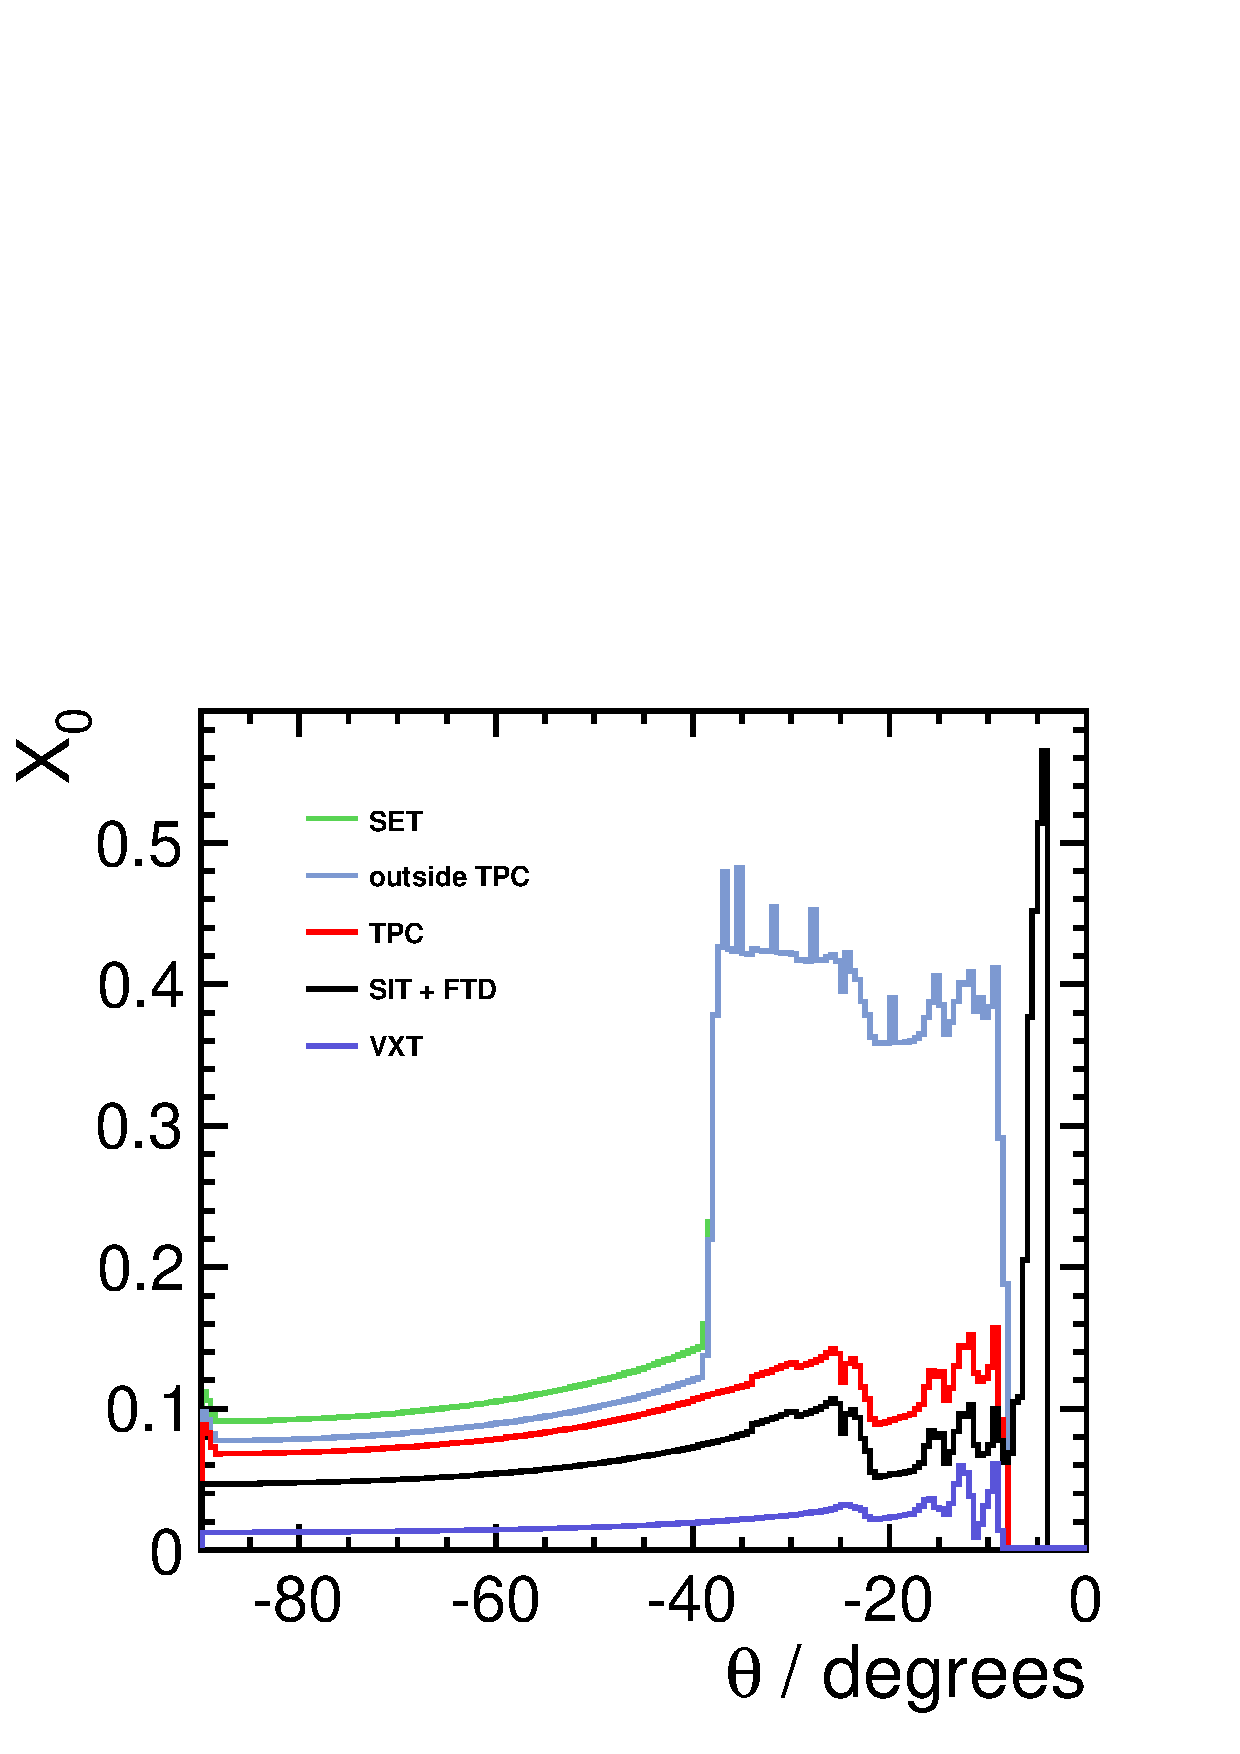
\includegraphics[width=0.52\hsize,viewport={0 -10 600 500},clip]{Introduction/fig/material-budget-new.pdf} &
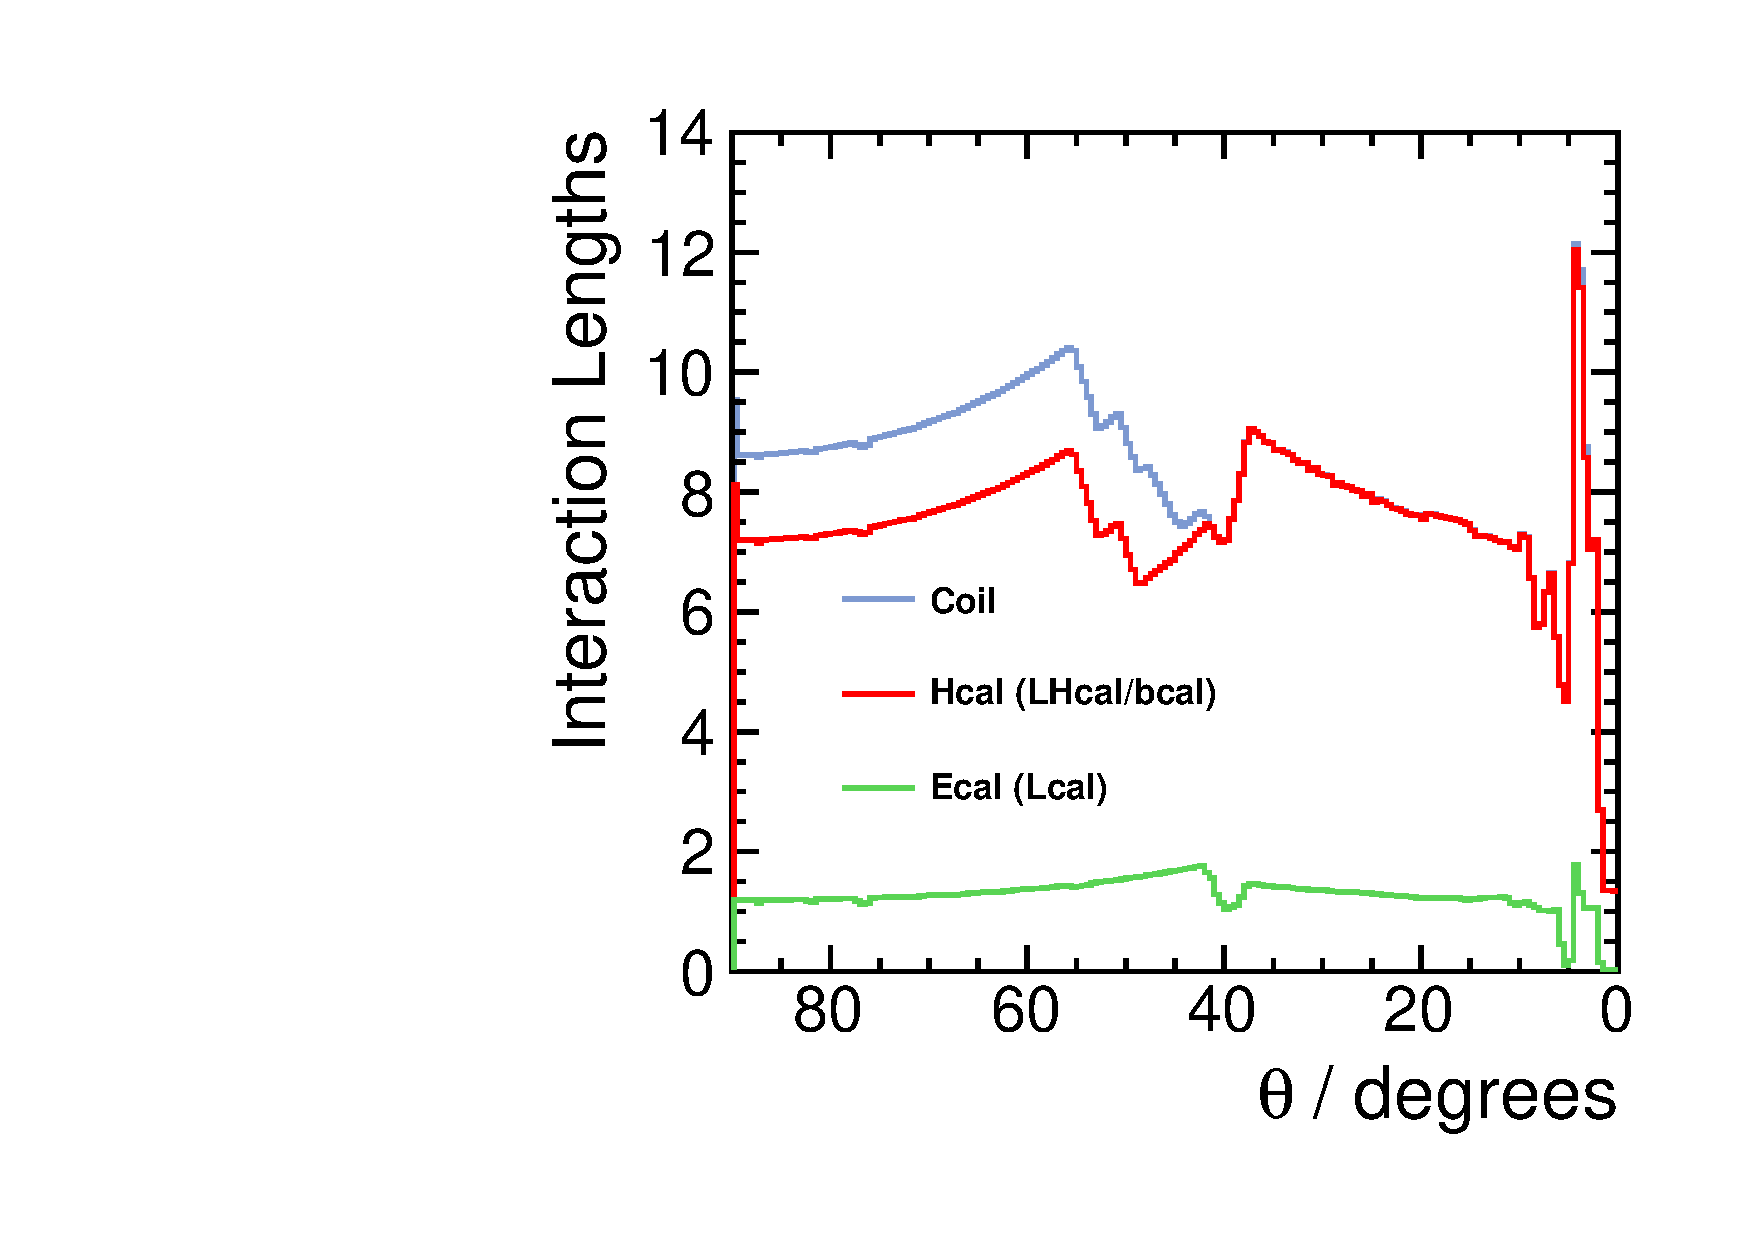
\includegraphics[width=0.5\hsize]{Introduction/fig/intlen_ILD_o1_v05.pdf}
\end{tabular}
\caption[Material in the ILD detector]{Left: Average total radiation length of the material
  in the tracking detectors as a function of polar angle. Right: Total interaction length in the detector, up to the end of the calorimeter system, and including the coil of the detector.}
%\end{figure}
\label{fig:intro:material}
%\begin{tabular}{cc}

\end{figure}


This is followed by a segmented hadronic calorimeter (HCAL) with up to 48 longitudinal samples and small transverse cell size. Two 
options are considered, both based on a Steel-absorber structure. One option uses scintillator tiles of $3 \times 3$\,cm$^2$, 
which are read out with an analogue system. The second uses a gas-based readout which allows a $1 \times 1$\,cm$^2$ 
cell geometry with a semi-digital readout of each cell. 

At very forward angles, below the coverage provided by the ECAL and the HCAL, a system of high precision and radiation hard calorimetric detectors (LumiCAL, BeamCAL, LHCAL) is foreseen. These
extend the calorimetric coverage to almost $4\pi$, measure the luminosity, and  monitor the quality of the colliding beams.

A large volume superconducting coil surrounds the calorimeters, creating an axial $B$-field of nominally 3.5-4\,Tesla.

An iron  yoke, instrumented with scintillator strips or resistive plate chambers (RPCs), returns the magnetic flux of the solenoid, and, at the same time, serves as a muon filter, muon detector and tail catcher calorimeter.

\thisfloatsetup{floatwidth=\SfigwFull,capposition=beside}
\begin{figure}[b!]
\begin{tabular}{cc}

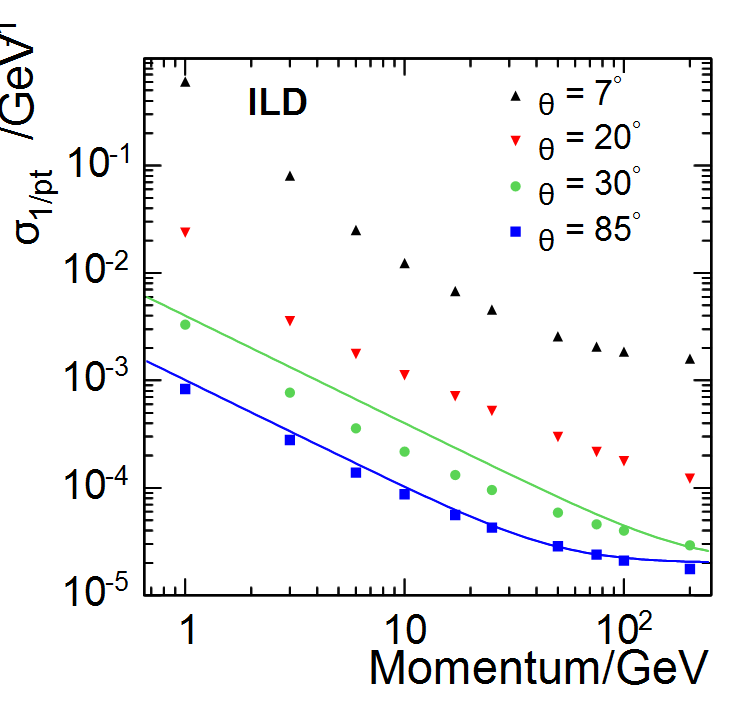
\includegraphics[width=0.5\hsize]{Introduction/fig/deltaInvP_all_fits.png} &
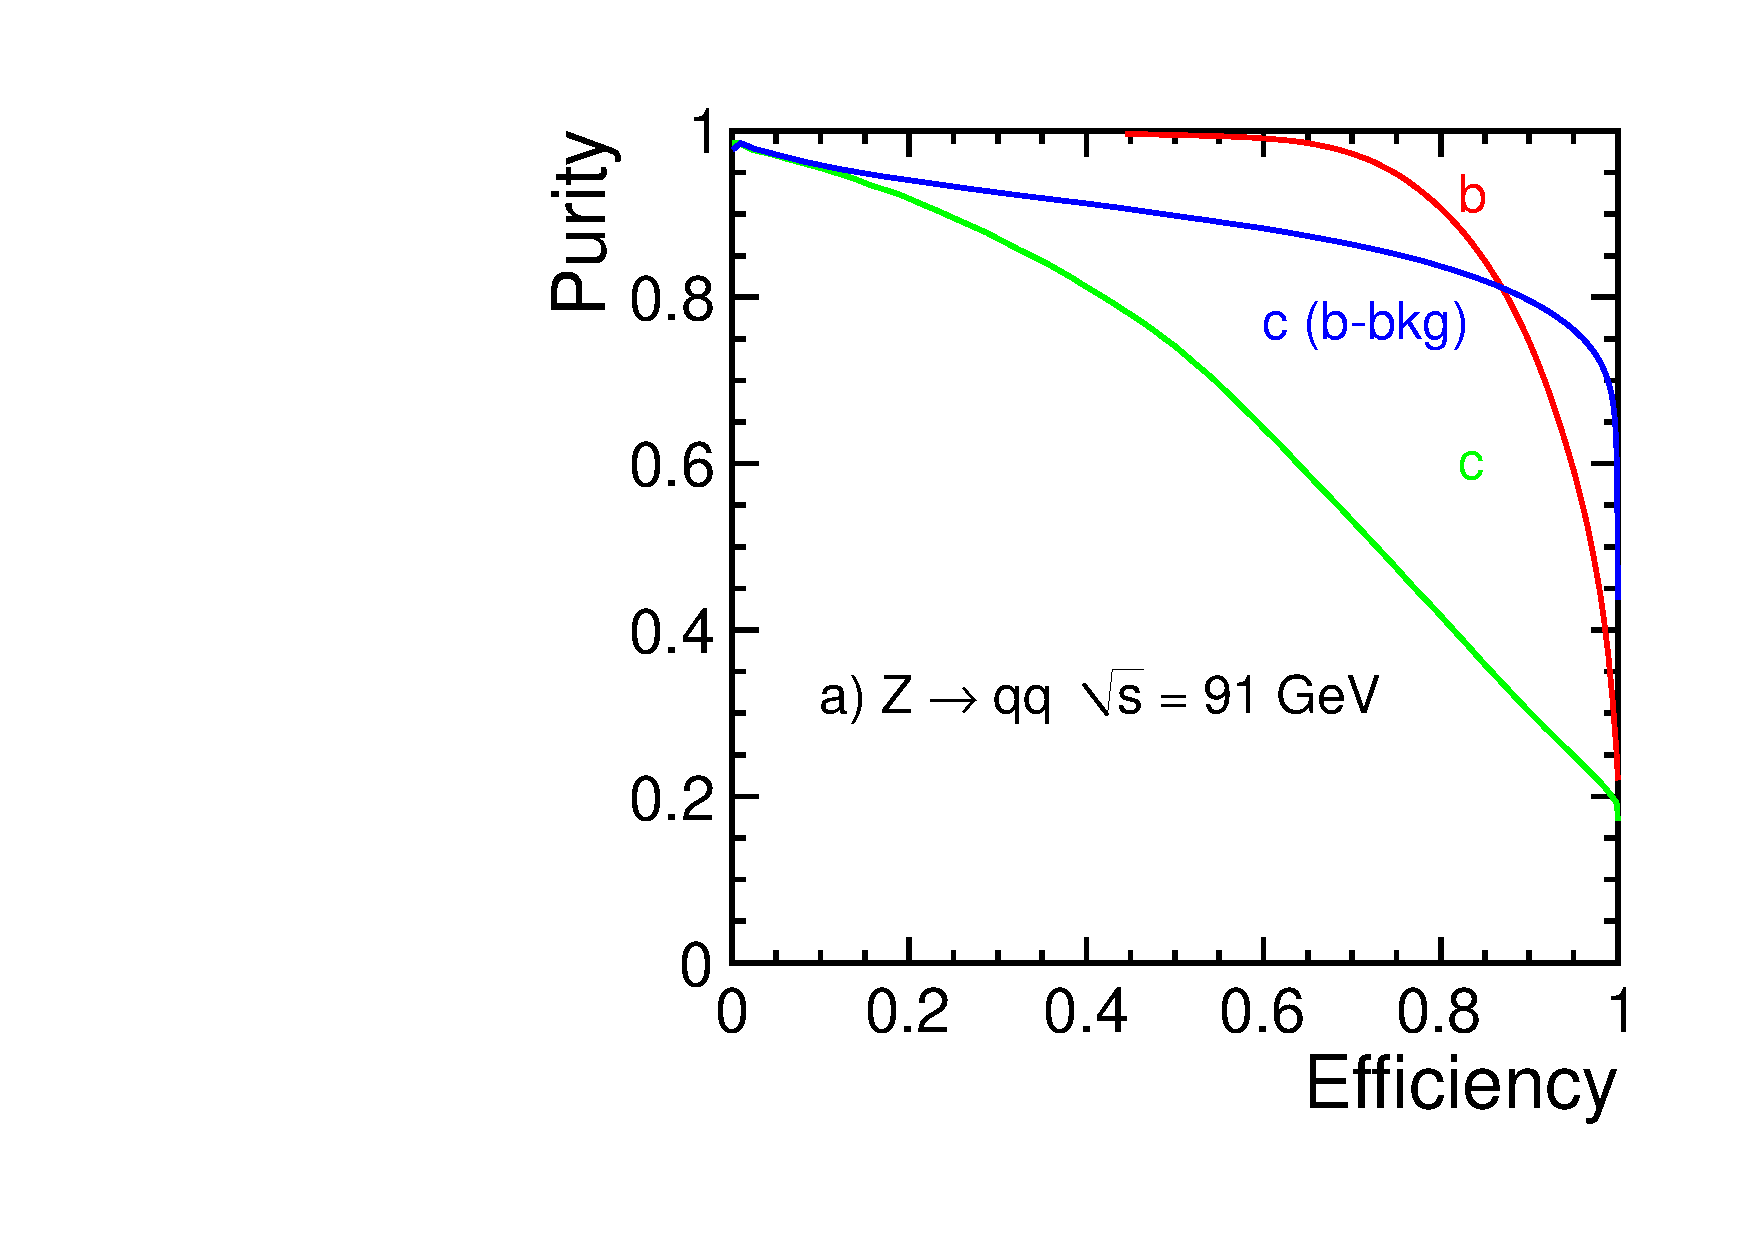
\includegraphics[width=0.5\hsize]{Introduction/fig/evalZ-lcfiweights_qq91new_v02-test.pdf}
\end{tabular}
\caption{\label{ild:fig:intro:tracking}(left) Momentum resolution for the ILD detector concept, as a function of the transverse momentum of the particle. (right) Flavour tagging efficiency versus purity for bottom events in sample of Z decays at 91\,GeV, and for charm events with only bottom background. )}
\end{figure}



\begin{figure}[t!]

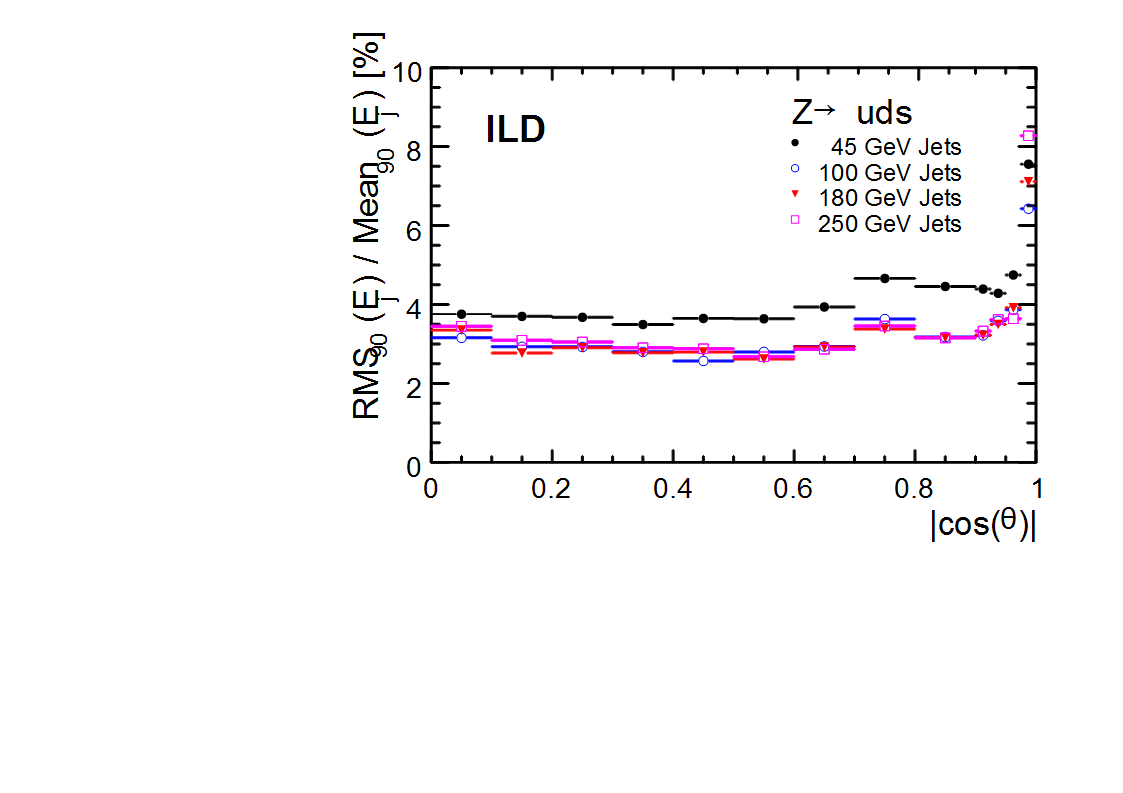
\includegraphics[width=0.8\hsize]{Introduction/fig/ild01_o1_pflow.png}

\caption{\label{ild:fig:intro:pflow}Fractional jet energy resolution
    plotted against $|\cos\theta|$ where theta is the polar angle of the thrust axis of the event. }
\end{figure}


The main parameters of the ILD detector are summarised in Table~\ref{ild:tab:barrelpara} and table~\ref{ild:tab:endcappara}.
%\begin{sidewaystable}[thb]
\begin{table}\hspace*{-0cm}\small
%\begin{tabular}{|l|p{0.8cm}p{0.8cm}p{1.0cm}|p{2.5cm}p{3.0cm}p{3.0cm}|}
%\begin{tabular}{|l|p{0.06\textwidth}p{0.06\textwidth}p{0.07\textwidth}|p{0.25\textwidth}p{0.20\textwidth}p{0.20\textwidth}|}
\begin{tabular}{ l p{0.05\hsize}p{0.04\hsize}p{0.04\hsize} p{0.20\hsize}p{0.20\hsize}p{0.20\hsize} }
%\hline
\toprule
\multicolumn{7}{l}{{\bf Barrel system}}\\
%\hline
\midrule
System & R(in) & R(out) & z & \multicolumn{3}{l}{comments}\\
       & \multicolumn{3}{c}{[mm]}   &&&\\
%\hline
\midrule
VTX    & 16         & 60        & 125 & 3 double layers &  Silicon pixel sensors, & \\
       &            &           &           & layer 1: & layer 2: & layer 3-6 \\
       &            &           &           & $\sigma<3 \mu m$ & $\sigma < 6 \mu m$ & $\sigma < 4 \mu m$ \\
Silicon &           &           & &&&\\
- SIT   & 153       & 300       & 644   & 2 silicon strip layers & $\sigma = 7 \mu m$& \\
- SET   & 1811      &           & 2300   & 2 silicon strip layers & $\sigma = 7 \mu m$& \\
- TPC   & 330       & 1808      & 2350   & MPGD readout & $1 \times 6 $mm$^2$ pads & $\sigma=60 \mu m$ at zero drift \\
%\hline
\midrule
ECAL    & 1843      & 2028      & 2350   & W absorber  & SiECAL & 30 Silicon sensor layers, $5 \times 5$ mm$^2$ cells \\
        &           &           &        &             & ScECAL & 30 Scintillator layers,  $ 5\times 45$ mm$^2$ strips \\
HCAL    & 2058      & 3410      & 2350   & Fe absorber & AHCAL & 48 Scintillator layers, $3 \times 3$cm$^2$ cells, analogue \\
        &           &           &         &            & SDHCAL & 48 Gas RPC layers, $1\times 1$ cm$^2$ cells, semi-digital\\
%\hline
\midrule
Coil    & 3440      & 4400      & 3950    & 3.5 T field & $ 2 \lambda $& \\
Muon    & 4450      & 7755      & 2800    & 14 scintillator layers& &\\
%\hline
\bottomrule
\end{tabular}
\caption{\label{ild:tab:barrelpara}List of the main parameters of the ILD detector for the barrel part.}
\end{table}

The performance of the ILD concept has been extensively studied using a detailed GEANT4 based simulation model and sophisticated reconstruction tools. Backgrounds have been taken into account to the best of current knowledge. 
A key characteristics of the detector is the amount of material in the detector. Particle flow requires a thin tracker, to minimise interactions before the calorimeters, and thick calorimeters, to fully absorb the showers. Figure~\ref{ild:fig:intro:material}~(left) shows the material in the detector in radiation lengths, until the entry of the calorimeter. The right plot shows the total interaction length including the calorimeter system. 

The performance of the tracking system can be summarised by its combined momentum resolution, shown in Figure~\ref{ild:fig:intro:tracking}~(left). A resolution of $\sigma_{1/p_T} = 2 \times 10^{-5}$\,GeV$^{-1}$ has been achieved for high momenta. For many physics studies the tagging of long lived particles is of key importance. Several layers of pixel detectors close to the IP allow the reconstruction of displaced vertices, as shown in Figure~\ref{ild:fig:intro:tracking}~(right).



%\begin{table}\hspace*{-2.5cm}\small
%\begin{tabular}{|l|p{0.8cm}p{0.8cm}p{1.0cm}|p{2.7cm}p{3.7cm}p{3.7cm}|}

\begin{table}\hspace*{-0cm}\small
%\begin{tabular}{|l|p{0.8cm}p{0.8cm}p{1.0cm}|p{2.5cm}p{3.0cm}p{3.0cm}|}
\begin{tabular}{ l p{0.05\hsize}p{0.04\hsize}p{0.04\hsize} p{0.20\hsize}p{0.20\hsize}p{0.20\hsize} }

%\hline
\toprule
\multicolumn{7}{ l }{{\bf End cap system}}\\
\midrule
System & z(min) & z(max) & r(min), r(max) & \multicolumn{3}{l}{comments}\\
       & \multicolumn{3}{c}{[mm]}   &&&\\
\midrule

FTD    & 220     & 371    &      & 2 pixel disks & $\sigma=2-6 \mu m$ &\\
       &         &        &      & 5 strip disks & $\sigma = 7 \mu m$& \\
ETD    & 2420    & 2445   & 419-1822 & 2 silicon strip layers & $\sigma=7 \mu m$ & \\
\midrule
ECAL   & 2450    & 2635   &      & W-absorber & SiECAL & Si readout layers \\
       &         &        &      &            & ScECAL & Scintillator layers \\
HCAL   & 2650    & 3937   & 335-3190& Fe absorber & AHCAL & 48 Scintillator layers $3 \times 3 $cm$^2$ cells, analogue\\
       &         &        &      &              & SDHCAL & 48 gas RPC layers $1\times 1$cm$^2$ cells, semi-digital \\
BeamCal & 3595   & 3715   & 20-150  & W absorber& 30 GaAs readout layers & \\
Lumical & 2500   & 2634   & 76-280 & W absorber & 30 Silicon layers & \\
LHCAL   & 2680   & 3205   & 93-331 & W absorber &&\\
\midrule
Muon    & 2560   &        & 300-7755 & 12 scintillator layers&&\\
\bottomrule
\end{tabular}
\caption{\label{ild:tab:endcappara}List of the main parameters of the ILD detector for the end cap part.}

\end{table}

Calorimeter system and tracking system together enter into the particle flow performance. The performance of the ILD detector for different energies and as a function of the polar angle is shown in Figure~\ref{ild:fig:intro:pflow}. 

The few plots shown in this introduction illustrate the anticipated performance of the detector and illustrate the potential for precision measurements with the ILD detector. More details on the performance may be found in section~\ref{ild:sec:performance} of this document. 

In this document the current state of the design of the ILD detector is summarised. The technologies which are proposed for the different parts of the detector are introduced. An extensive benchmarking has been performed, to demonstrate the performance of the ILD detector. This has been done for two different detector implementations, a large and a smaller one. Both concepts are the result of intense optimization efforts, with different goals - cost effectivnes was foremost a criterium for the smaller one, ultimate performance for the larger model. 

The ILD group who is proposing this detector has currently some 70 member institutes from all around the world. The group has evolved into a proto-collaboration, which is positioning itself to move forward with a proposal for a detector at the ILC at the moment that ILC becomes a real project. 

A lot of the work presented in this report is based on intense R\&D work which has taken place over the last decade to develop the necessary technologies. 
This work has typically happened within dedicated R\&D collaborations, which are independent but maintain very close connections to ILD. All technologies selected by ILD for one of its subsystems have been proven experimentally to meet the performance goals, or to come very close. 

Developing a very powerful detector concept over a long period of time requires balancing cutting edge technologies, which might become available while the concept is being developed, with safe and sound solutions. ILD in many cases is pursuing more than one technological option, to remain flexible and to be able to adopt to new developments. The concept group  wants to remain open and flexible to be prepared to select the most modern and most powerful technology once it is necessary. 
However a distinction is made between options and alternatives: while options have undergone an extensive R\&D program and have passed critical proof-of-concept tests, alternatives are potentially interesting and promising technologies which have not matured to a similar level at the time of writing this document. 

The following document starts with a short review of the science goals of the ILC, and how the goals can be achieved today with the detector technologies at hand. After a discussion of the ILC and the environment in which the experiment will take place the detector is described in more detail. The integration of the different sub-systems into an integrated detector is discussed, as is the interface between the detector and the collider. This is followed by a concise summary of the benchmarking which has been performed in order to find an optimal balance between performance and cost. To this end the costing methodology used by ILD is presented, and a cost estimate for the detector in 2018 costs is presented. The report closes with a summary of the proposed detector and its performance. 